29. \begin{figure}[ht!]
\center{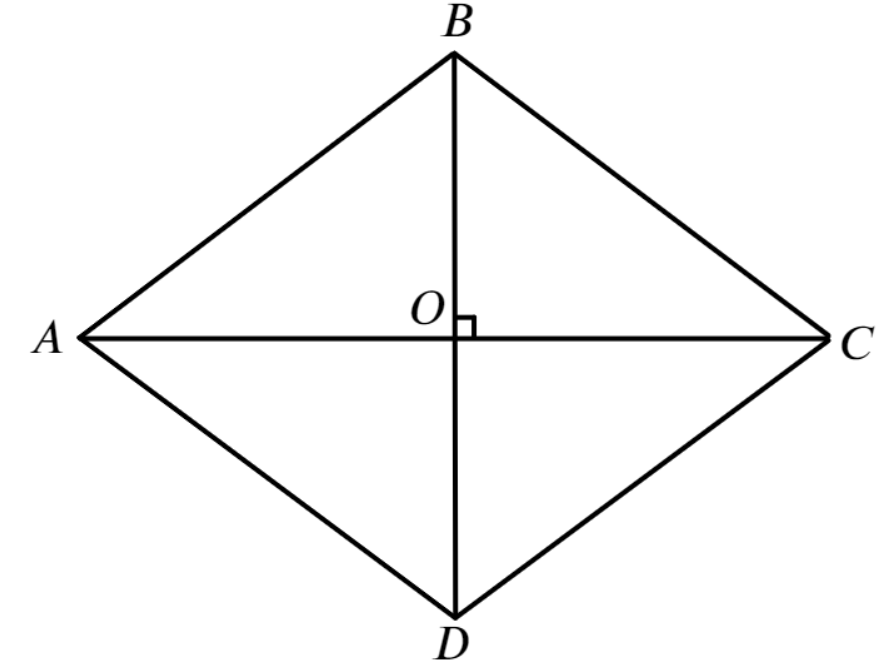
\includegraphics[scale=0.35]{g9-29.png}}
\end{figure}\\
В ромбе диагонали перпендикулярны и делятся точкой пересечения пополам. Если $BD=12$см, то по теореме Пифагора $AO=\sqrt{100-36}=8$см, значит вторая диагональ равна 16 см. Площадь ромба равна половине произведения диагоналей, значит $S=\cfrac{1}{2}\cdot12\cdot16=96\text{ см}^2.$\\
